
%\documentclass[11pts,a4paper,amsmath,amssymb,floatfix]{article}%{report}%{book}
\documentclass[12pts,a4paper,amsmath,amssymb,floatfix]{article}%{report}%{book}
\usepackage{graphicx,wrapfig,pdfpages}% Include figure files
%\usepackage{dcolumn,enumerate}% Align table columns on decimal point
\usepackage{enumerate,enumitem}% Align table columns on decimal point
\usepackage{bm,dpfloat}% bold math
\usepackage[pdftex,bookmarks,colorlinks=true,urlcolor=rltblue,citecolor=blue]{hyperref}
\usepackage{amsfonts,amsmath,amssymb,stmaryrd,indentfirst}
\usepackage{times,psfrag}
\usepackage{natbib}
\usepackage{color}
\usepackage{units}
\usepackage{rotating}
\usepackage{multirow}


\usepackage{pifont}
\usepackage{subfigure}
\usepackage{subeqnarray}
\usepackage{ifthen}

\usepackage{supertabular}
\usepackage{moreverb}
\usepackage{listings}
\usepackage{palatino}
%\usepackage{doi}
\usepackage{longtable}
\usepackage{float}
\usepackage{perpage}
\MakeSorted{figure}
%\usepackage{pdflscape}


%\usepackage{booktabs}
%\newcommand{\ra}[1]{\renewcommand{\arraystretch}{#1}}


\definecolor{rltblue}{rgb}{0,0,0.75}


%\usepackage{natbib}
\usepackage{fancyhdr} %%%%
\pagestyle{fancy}%%%%
% with this we ensure that the chapter and section
% headings are in lowercase
%%%%\renewcommand{\chaptermark}[1]{\markboth{#1}{}}
\renewcommand{\sectionmark}[1]{\markright{\thesection\ #1}}
\fancyhf{} %delete the current section for header and footer
\fancyhead[LE,RO]{\bfseries\thepage}
\fancyhead[LO]{\bfseries\rightmark}
\fancyhead[RE]{\bfseries\leftmark}
\renewcommand{\headrulewidth}{0.5pt}
% make space for the rule
\fancypagestyle{plain}{%
\fancyhead{} %get rid of the headers on plain pages
\renewcommand{\headrulewidth}{0pt} % and the line
}

\def\newblock{\hskip .11em plus .33em minus .07em}
\usepackage{color}

%\usepackage{makeidx}
%\makeindex

\setlength\textwidth      {16.cm}
\setlength\textheight     {22.6cm}
\setlength\oddsidemargin  {-0.3cm}
\setlength\evensidemargin {0.3cm}

\setlength\headheight{14.49998pt} 
\setlength\topmargin{0.0cm}
\setlength\headsep{1.cm}
\setlength\footskip{1.cm}
\setlength\parskip{0pt}
\setlength\parindent{0pt}


%%%
%%% Headers and Footers
\lhead[] {\text{\small{EG3521 -- Engineering Thermodynamics}}} 
\rhead[] {{\text{\small{Tutorial 05 (2014/15)}}}}
%\chead[] {\text{\small{Session 2012/13}}} 
\lfoot[]{Dr Jeff Gomes}
%\cfoot[\thepage]{\thepage}
\rfoot[\text{\small{\thepage}}]{\thepage}
\renewcommand{\headrulewidth}{0.8pt}


%%%
%%% space between lines
%%%
\renewcommand{\baselinestretch}{1.5}

\newenvironment{VarDescription}[1]%
  {\begin{list}{}{\renewcommand{\makelabel}[1]{\textbf{##1:}\hfil}%
    \settowidth{\labelwidth}{\textbf{#1:}}%
    \setlength{\leftmargin}{\labelwidth}\addtolength{\leftmargin}{\labelsep}}}%
  {\end{list}}

%%%%%%%%%%%%%%%%%%%%%%%%%%%%%%%%%%%%%%%%%%%
%%%%%%                              %%%%%%%
%%%%%%      NOTATION SECTION        %%%%%%%
%%%%%%                              %%%%%%%
%%%%%%%%%%%%%%%%%%%%%%%%%%%%%%%%%%%%%%%%%%%

% Text abbreviations.
\newcommand{\ie}{{\em{i.e., }}}
\newcommand{\eg}{{\em{e.g., }}}
\newcommand{\cf}{{\em{cf., }}}
\newcommand{\wrt}{with respect to}
\newcommand{\lhs}{left hand side}
\newcommand{\rhs}{right hand side}
% Commands definining mathematical notation.

% This is for quantities which are physically vectors.
\renewcommand{\vec}[1]{{\mbox{\boldmath$#1$}}}
% Physical rank 2 tensors
\newcommand{\tensor}[1]{\overline{\overline{#1}}}
% This is for vectors formed of the value of a quantity at each node.
\newcommand{\dvec}[1]{\underline{#1}}
% This is for matrices in the discrete system.
\newcommand{\mat}[1]{\mathrm{#1}}


\DeclareMathOperator{\sgn}{sgn}
\newtheorem{thm}{Theorem}[section]
\newtheorem{lemma}[thm]{Lemma}

%\newcommand\qed{\hfill\mbox{$\Box$}}
\newcommand{\re}{{\mathrm{I}\hspace{-0.2em}\mathrm{R}}}
\newcommand{\inner}[2]{\langle#1,#2\rangle}
\renewcommand\leq{\leqslant}
\renewcommand\geq{\geqslant}
\renewcommand\le{\leqslant}
\renewcommand\ge{\geqslant}
\renewcommand\epsilon{\varepsilon}
\newcommand\eps{\varepsilon}
\renewcommand\phi{\varphi}
\newcommand{\bmF}{\vec{F}}
\newcommand{\bmphi}{\vec{\phi}}
\newcommand{\bmn}{\vec{n}}
\newcommand{\bmns}{{\textrm{\scriptsize{\boldmath $n$}}}}
\newcommand{\bmi}{\vec{i}}
\newcommand{\bmj}{\vec{j}}
\newcommand{\bmk}{\vec{k}}
\newcommand{\bmx}{\vec{x}}
\newcommand{\bmu}{\vec{u}}
\newcommand{\bmv}{\vec{v}}
\newcommand{\bmr}{\vec{r}}
\newcommand{\bma}{\vec{a}}
\newcommand{\bmg}{\vec{g}}
\newcommand{\bmU}{\vec{U}}
\newcommand{\bmI}{\vec{I}}
\newcommand{\bmq}{\vec{q}}
\newcommand{\bmT}{\vec{T}}
\newcommand{\bmM}{\vec{M}}
\newcommand{\bmtau}{\vec{\tau}}
\newcommand{\bmOmega}{\vec{\Omega}}
\newcommand{\pp}{\partial}
\newcommand{\kaptens}{\tensor{\kappa}}
\newcommand{\tautens}{\tensor{\tau}}
\newcommand{\sigtens}{\tensor{\sigma}}
\newcommand{\etens}{\tensor{\dot\epsilon}}
\newcommand{\ktens}{\tensor{k}}
\newcommand{\half}{{\textstyle \frac{1}{2}}}
\newcommand{\tote}{E}
\newcommand{\inte}{e}
\newcommand{\strt}{\dot\epsilon}
\newcommand{\modu}{|\bmu|}
% Derivatives
\renewcommand{\d}{\mathrm{d}}
\newcommand{\D}{\mathrm{D}}
\newcommand{\ddx}[2][x]{\frac{\d#2}{\d#1}}
\newcommand{\ddxx}[2][x]{\frac{\d^2#2}{\d#1^2}}
\newcommand{\ddt}[2][t]{\frac{\d#2}{\d#1}}
\newcommand{\ddtt}[2][t]{\frac{\d^2#2}{\d#1^2}}
\newcommand{\ppx}[2][x]{\frac{\partial#2}{\partial#1}}
\newcommand{\ppxx}[2][x]{\frac{\partial^2#2}{\partial#1^2}}
\newcommand{\ppt}[2][t]{\frac{\partial#2}{\partial#1}}
\newcommand{\pptt}[2][t]{\frac{\partial^2#2}{\partial#1^2}}
\newcommand{\DDx}[2][x]{\frac{\D#2}{\D#1}}
\newcommand{\DDxx}[2][x]{\frac{\D^2#2}{\D#1^2}}
\newcommand{\DDt}[2][t]{\frac{\D#2}{\D#1}}
\newcommand{\DDtt}[2][t]{\frac{\D^2#2}{\D#1^2}}
% Norms
\newcommand{\Ltwo}{\ensuremath{L_2} }
% Basis functions
\newcommand{\Qone}{\ensuremath{Q_1} }
\newcommand{\Qtwo}{\ensuremath{Q_2} }
\newcommand{\Qthree}{\ensuremath{Q_3} }
\newcommand{\QN}{\ensuremath{Q_N} }
\newcommand{\Pzero}{\ensuremath{P_0} }
\newcommand{\Pone}{\ensuremath{P_1} }
\newcommand{\Ptwo}{\ensuremath{P_2} }
\newcommand{\Pthree}{\ensuremath{P_3} }
\newcommand{\PN}{\ensuremath{P_N} }
\newcommand{\Poo}{\ensuremath{P_1P_1} }
\newcommand{\PoDGPt}{\ensuremath{P_{-1}P_2} }

\newcommand{\metric}{\tensor{M}}
\newcommand{\configureflag}[1]{\texttt{#1}}

% Units
\newcommand{\m}[1][]{\unit[#1]{m}}
\newcommand{\km}[1][]{\unit[#1]{km}}
\newcommand{\s}[1][]{\unit[#1]{s}}
\newcommand{\invs}[1][]{\unit[#1]{s}\ensuremath{^{-1}}}
\newcommand{\ms}[1][]{\unit[#1]{m\ensuremath{\,}s\ensuremath{^{-1}}}}
\newcommand{\mss}[1][]{\unit[#1]{m\ensuremath{\,}s\ensuremath{^{-2}}}}
\newcommand{\K}[1][]{\unit[#1]{K}}
\newcommand{\PSU}[1][]{\unit[#1]{PSU}}
\newcommand{\Pa}[1][]{\unit[#1]{Pa}}
\newcommand{\kg}[1][]{\unit[#1]{kg}}
\newcommand{\rads}[1][]{\unit[#1]{rad\ensuremath{\,}s\ensuremath{^{-1}}}}
\newcommand{\kgmm}[1][]{\unit[#1]{kg\ensuremath{\,}m\ensuremath{^{-2}}}}
\newcommand{\kgmmm}[1][]{\unit[#1]{kg\ensuremath{\,}m\ensuremath{^{-3}}}}
\newcommand{\Nmm}[1][]{\unit[#1]{N\ensuremath{\,}m\ensuremath{^{-2}}}}

% Dimensionless numbers
\newcommand{\dimensionless}[1]{\mathrm{#1}}
\renewcommand{\Re}{\dimensionless{Re}}
\newcommand{\Ro}{\dimensionless{Ro}}
\newcommand{\Fr}{\dimensionless{Fr}}
\newcommand{\Bu}{\dimensionless{Bu}}
\newcommand{\Ri}{\dimensionless{Ri}}
\renewcommand{\Pr}{\dimensionless{Pr}}
\newcommand{\Pe}{\dimensionless{Pe}}
\newcommand{\Ek}{\dimensionless{Ek}}
\newcommand{\Gr}{\dimensionless{Gr}}
\newcommand{\Ra}{\dimensionless{Ra}}
\newcommand{\Sh}{\dimensionless{Sh}}
\newcommand{\Sc}{\dimensionless{Sc}}


% Journals
\newcommand{\IJHMT}{{\it International Journal of Heat and Mass Transfer}}
\newcommand{\NED}{{\it Nuclear Engineering and Design}}
\newcommand{\ICHMT}{{\it International Communications in Heat and Mass Transfer}}
\newcommand{\NET}{{\it Nuclear Engineering and Technology}}
\newcommand{\HT}{{\it Heat Transfer}}   
\newcommand{\IJHT}{{\it International Journal for Heat Transfer}}

\newcommand{\frc}{\displaystyle\frac}

\newlist{ExList}{enumerate}{1}
\setlist[ExList,1]{label={\bf Example 1.} {\bf \arabic*}}

\newlist{ProbList}{enumerate}{1}
\setlist[ProbList,1]{label={\bf Problem 1.} {\bf \arabic*}}

%%%%%%%%%%%%%%%%%%%%%%%%%%%%%%%%%%%%%%%%%%%
%%%%%%                              %%%%%%%
%%%%%% END OF THE NOTATION SECTION  %%%%%%%
%%%%%%                              %%%%%%%
%%%%%%%%%%%%%%%%%%%%%%%%%%%%%%%%%%%%%%%%%%%


% Cause numbering of subsubsections. 
%\setcounter{secnumdepth}{8}
%\setcounter{tocdepth}{8}

\setcounter{secnumdepth}{4}%
\setcounter{tocdepth}{4}%


\begin{document}


\begin{enumerate}[label=\bfseries Problem \arabic*]

%%%
%%% EXAMPLE
%%%
\item For the heating of a residence in a cold enviroment (-5$^{\text{o}}$C), a heat pump was used. The engine was designed to maintain the house's interior temperature at 25$^{\text{o}}$C. The compressor heat pump is driven by a heat engine working between 1000$^{\text{o}}$C and 25$^{\text{o}}$C. Assume that both cycles are reversibles, determine the ratio in which the heat pump and the heat engine share the heating load.

%%%
%%% EXAMPLE
%%%
\item A refrigerating engine operates on the Bell-Coleman cycle (of 6 tonnes capacity) with upper limiting pressure of 5.2 bar. Pressure and temperature at the beginning of the compression stage are 1.0 bar and 16$^{\text{o}}$C, respectively. The compressed air is cooled at constant pressure from a temperature of 41$^{\text{o}}$C  (flow entering the expansion cylinder). Assuming that both expansion and compression processes are adiabatic with $\gamma=1.4$ and the latent heat of fusion of water $\left(\text{L}_{\text{f}}\right)$ is 336 kJ/kg determine:

\begin{enumerate}
\item COP;
\item Mass flow rate of air in circulation (kg/min);
\item Piston displacement of compressor and expander, bore of compressor and expansion cylinders. The unit runs at 240 rpm. Assume that the stroke length is 200 mm;
\item Power required to drive the unit.
\end{enumerate}

%%%
%%% Rajput (pg 739-40)
%%%
\item \label{Ex4} Derive the clearance volumetric efficiency $\left(\eta_{cv}\right)$ expression in a compressor (Fig. \ref{ex4_pic}) assuming polytropic expansion.
\begin{figure}[h]
 \begin{center}
  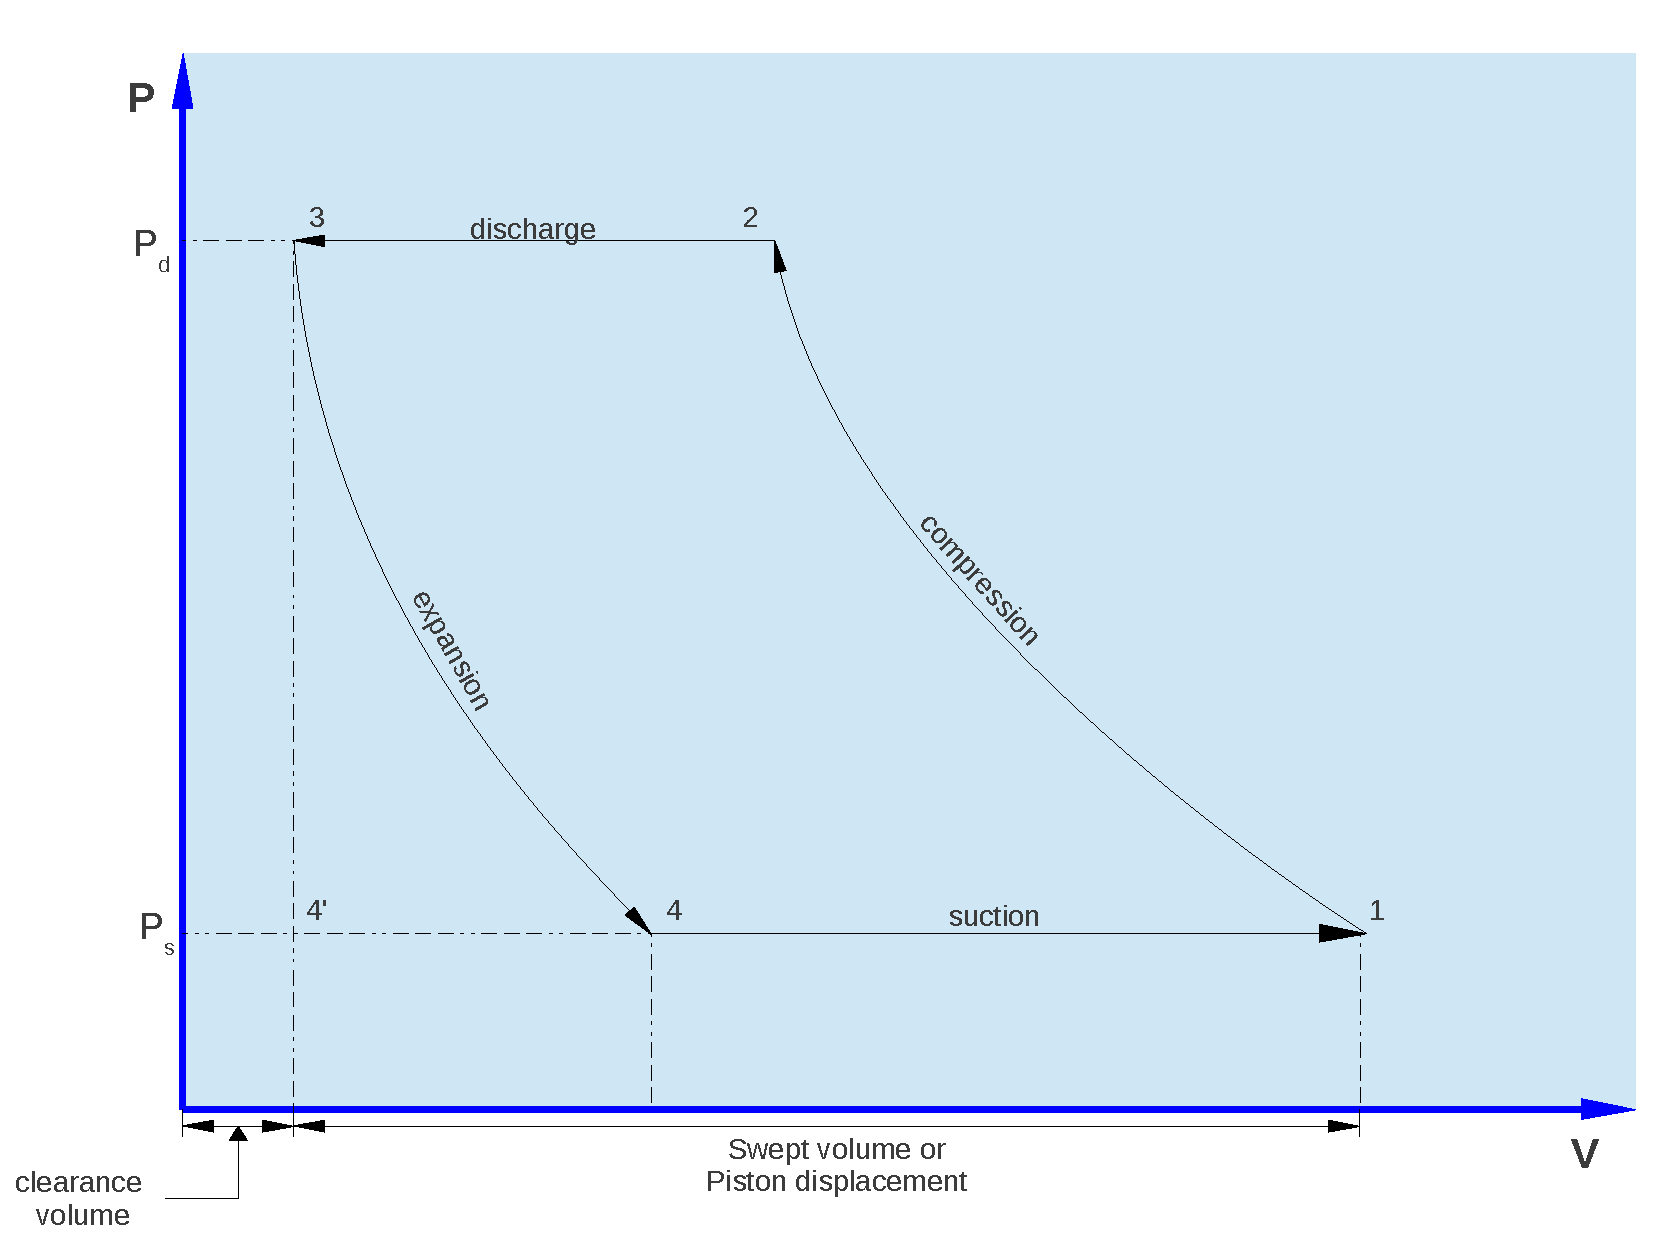
\includegraphics[width=12.cm,height=8.cm,clip]{./Pics/Overview_Refrig29}
  \end{center}
  \caption{Strokes in the compressor: Problem \ref{Ex4}.}\label{ex4_pic}
\end{figure}  


%%%
%%% Shapiro 9.49
%%%
\item Air enters the compressor of a cold air-standard Brayton ycle at 100 kPa, 300 K, with a mass flow rate of 6 kg.s$^{-1}$. The compressor pressure ratio is 10, and the turbine inlet temperature is 1400 K. The turbine and compressor each have isentropic efficiencies of 80$\%$. Calculate:
\begin{enumerate}
\item Thermal efficiency of the cycle;
\item Net power (in kW).
\end{enumerate}


%%%
%%% Ameen (example 3.3, pg 50)
%%%
\item \label{Ex5} An ice plant operates on the ideal vapour-compression cycle with superheated state using refrigerant fluid R134a.  The refrigerant enters the compressor as saturated vapour at 0.15 MPa and leaves the condenser as saturated liquid at 0.7 MPa.  Water enters the refrigerator cavity at 30$^{\text{o}}$C and leaves as ice at -5$^{\text{o}}$C. For an ice production rate of 10 kg per hour, determine the power input to the ice plant and the COP of the cycle. Also, sketch the $PH$ and $TS$ diagrams. Specific heats of ice and water are 2.1 and 4.18 kJ/(kg.K), respectively, and the latent heat of fusion of ice is 334 kJ/kg. Repeat the same procedure for ammonia and propane as refrigerat fluid.



%%%
%%% Rajput Ex 14.24
%%%
\item \label{Ex10} A heat pump operates in a vapour-compression cycle using Refrigerant-22 (R-22) as working fluid.  R-22 is compressed from saturated vapour at 2 bar to the condenser pressure of 12 bar.  The isentropic efficiency of the compressor is of 80$\%$. Saturated liquid enters the throttling valve at 12 bar. 80$\%$ of the heat rejected is transferred to the heated space which has a total heating requirement of 500 kJ/min. Determine:
\begin{enumerate}
\item (A)-(H) in the Table below:

%\begin{table}[h]
\begin{center}
\begin{tabular}{ || c || c | c | c | c || }
\hline\hline
        & {\bf Pressure}  &  {\bf Enthalpy}  & {\bf Entropy}     & {\bf State}  \\
        & {\bf (bar)}     &  {\bf (kJ/kg)}   &  {\bf (kJ/kg.K)}  &              \\
\hline\hline
{\bf 1} &   2.0           &       (A)        &      (B)          &  Saturated Vapour \\
{\bf 2} &   12.0          &       (C)        &      --           &  (D)          \\
{\bf 3} &   12.0          &       (E)        &      --           &  (F)        \\
{\bf 4} &   --            &       (G)        &      --           &  (H)       \\ 
\hline\hline
\end{tabular}
\end{center}
%\end{table}

\item Mass flow rate of the R-22 in kg/min.
\item Actual work in the compressor.
\item Coefficient of performance.

\end{enumerate}


%%%
%%% Shapiro 10.42
%%%
\item \label{Ex13} R-22 is the refrigerant fluid in a geothermal heat pump system for a house (Fig. \ref{Ex13:Fig}). The heat pump uses underground water from a well $\left(T_{\text{w}}^{\text{in}}=13^{\text{o}}\text{C}; T_{\text{w}}^{\text{out}}=7^{\text{o}}\text{C}\right)$ to produce a heating capacity of 4.2 tons. Determine:
\begin{enumerate}
 \item Volumetric flow rate of heated air to the house $\left(m^{3}/s\right)$;
 \item Isentropic efficiency $\left(\eta_{c}\right)$ and power $\left(\dot{W}_{c}\right)$ of the compressor;
 \item Coefficient of Performance;
 \item Volumetric flow rate of water from the geothermal well $\left(l/h\right)$;
 \item Sketch the $TS$ diagram.
\end{enumerate}
Given the heat capacity $\left(C_{p}^{\text{air}}=1.004\displaystyle\frac{kJ}{kg.K}\right)$ and molecular weight $\left(MW^{\text{air}}=28.97\displaystyle\frac{kg}{kgmol}\right)$ of air and heat capacity of water $\left(C_{p}^{\text{water}}=4.1813\displaystyle\frac{kJ}{kg.K}\right)$.

\begin{figure}[h]
\begin{center}
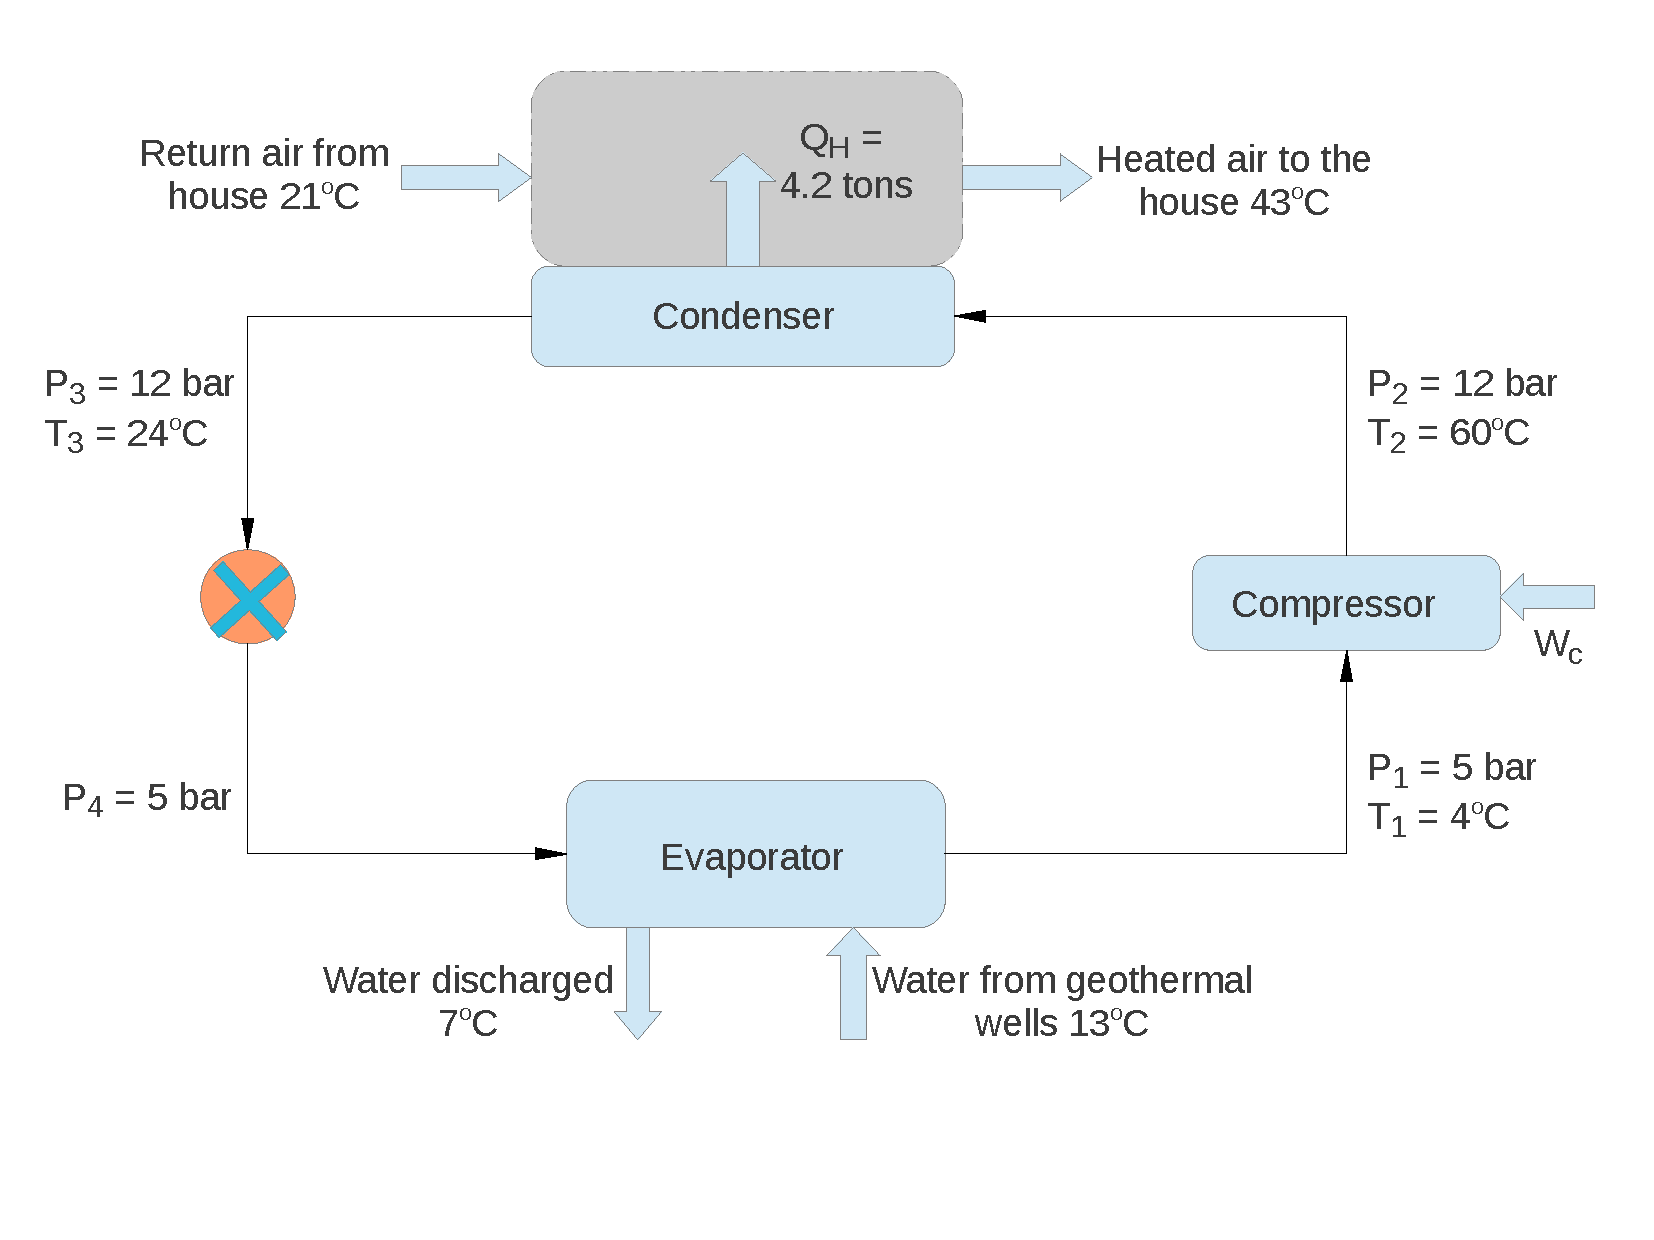
\includegraphics[width=16.0cm,height=12.0cm]{./Pics/Overview_Refrig42}
\end{center}
\caption{Heat pump cycle: Problem \ref{Ex13}.}\label{Ex13:Fig}
\end{figure}
 
\end{enumerate}



\end{document}
 
